% Source: StudentGovernmentRepo/Common_Sense_Carolina_Lobbying_org/figures/org_phase2.tex
\documentclass[border=5pt]{standalone}
\usepackage{tikz}
\usepackage{xcolor}
\usetikzlibrary{arrows.meta}

\definecolor{garnet}{HTML}{73000A}
\definecolor{rose}{HTML}{CC2E40}
\definecolor{atlantic}{HTML}{466A9F}
\definecolor{congaree}{HTML}{1F414D}
\definecolor{horseshoe}{HTML}{65780B}

\begin{document}
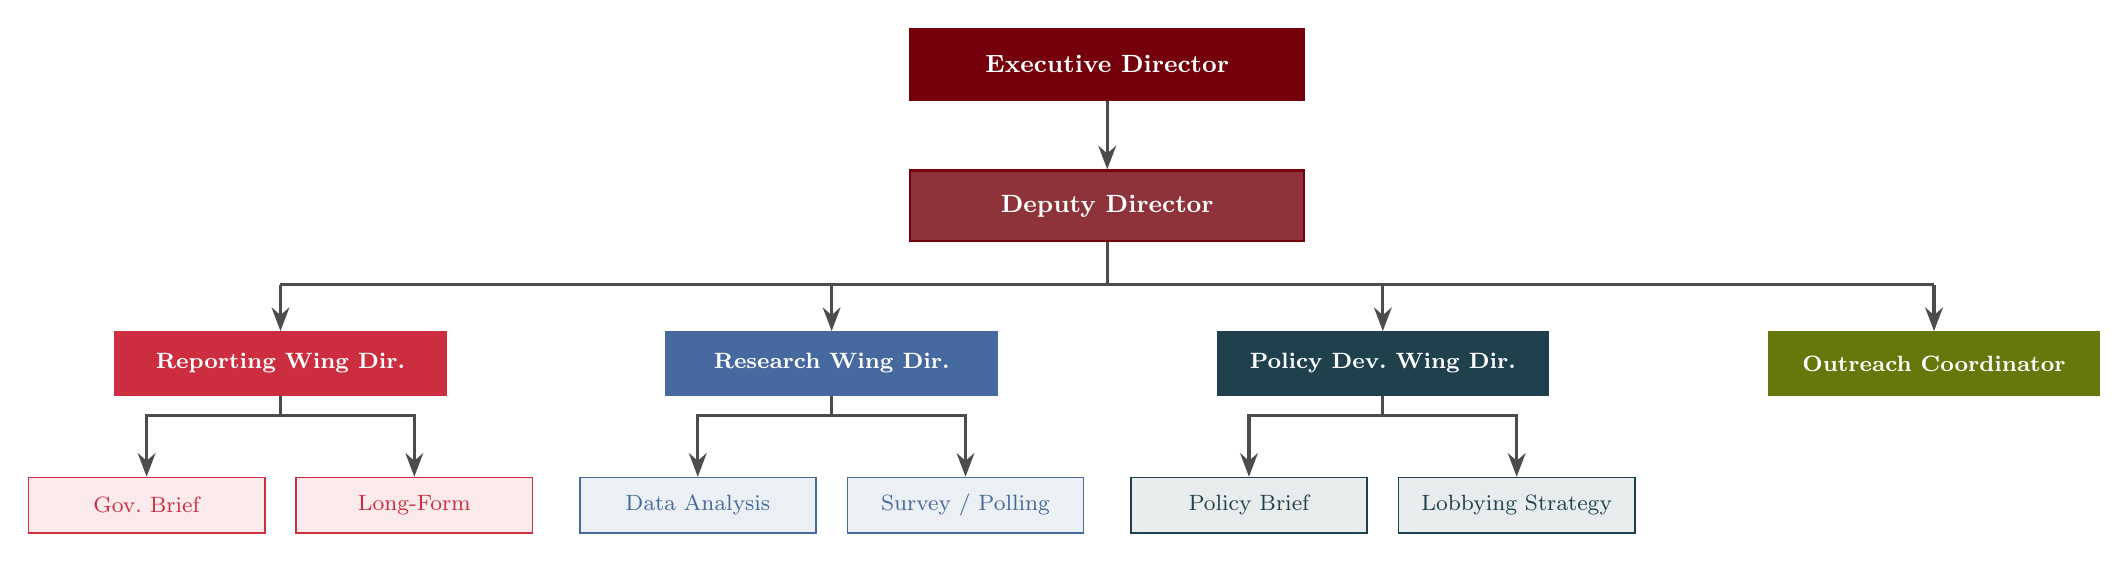
\begin{tikzpicture}[
  every node/.style={rectangle, sharp corners, align=center},
  arrow/.style={-{Stealth[length=3mm]}, line width=1.2pt, black!70}
]

%% Row 0: Executive Director
\node[
  fill=garnet, text=white, draw=garnet, line width=0.8pt,
  font=\small\bfseries,
  minimum width=5cm, minimum height=0.9cm
] (exec) at (0,0) {Executive Director};

%% Row 1: Deputy Director
\node[
  fill=garnet!80, text=white, draw=garnet, line width=0.8pt,
  font=\small\bfseries,
  minimum width=5cm, minimum height=0.9cm
] (deputy) at (0,-1.8) {Deputy Director};

%% Row 2: Wing Directors + Outreach (7cm spacing)
\node[
  fill=rose, text=white, draw=rose, line width=0.6pt,
  font=\footnotesize\bfseries,
  minimum width=4.2cm, minimum height=0.8cm
] (report) at (-10.5,-3.8) {Reporting Wing Dir.};

\node[
  fill=atlantic, text=white, draw=atlantic, line width=0.6pt,
  font=\footnotesize\bfseries,
  minimum width=4.2cm, minimum height=0.8cm
] (research) at (-3.5,-3.8) {Research Wing Dir.};

\node[
  fill=congaree, text=white, draw=congaree, line width=0.6pt,
  font=\footnotesize\bfseries,
  minimum width=4.2cm, minimum height=0.8cm
] (policy) at (3.5,-3.8) {Policy Dev.\ Wing Dir.};

\node[
  fill=horseshoe, text=white, draw=horseshoe, line width=0.6pt,
  font=\footnotesize\bfseries,
  minimum width=4.2cm, minimum height=0.8cm
] (outreach) at (10.5,-3.8) {Outreach Coordinator};

%% Row 3: Sub-units (1.7cm offset, well separated between groups)
% Under Reporting (-10.5)
\node[
  fill=rose!10, draw=rose, text=rose, line width=0.6pt,
  font=\footnotesize,
  minimum width=3cm, minimum height=0.7cm
] (govbrief) at (-12.2,-5.6) {Gov.\ Brief};

\node[
  fill=rose!10, draw=rose, text=rose, line width=0.6pt,
  font=\footnotesize,
  minimum width=3cm, minimum height=0.7cm
] (longform) at (-8.8,-5.6) {Long-Form};

% Under Research (-3.5)
\node[
  fill=atlantic!10, draw=atlantic, text=atlantic, line width=0.6pt,
  font=\footnotesize,
  minimum width=3cm, minimum height=0.7cm
] (data) at (-5.2,-5.6) {Data Analysis};

\node[
  fill=atlantic!10, draw=atlantic, text=atlantic, line width=0.6pt,
  font=\footnotesize,
  minimum width=3cm, minimum height=0.7cm
] (survey) at (-1.8,-5.6) {Survey / Polling};

% Under Policy (3.5)
\node[
  fill=congaree!10, draw=congaree, text=congaree, line width=0.6pt,
  font=\footnotesize,
  minimum width=3cm, minimum height=0.7cm
] (policybrief) at (1.8,-5.6) {Policy Brief};

\node[
  fill=congaree!10, draw=congaree, text=congaree, line width=0.6pt,
  font=\footnotesize,
  minimum width=3cm, minimum height=0.7cm
] (lobbying) at (5.2,-5.6) {Lobbying Strategy};

%% Arrows — Row 0 to Row 1
\draw[arrow] (exec) -- (deputy);

%% Arrows — Deputy to Wing Directors (T-junction)
%% Vertical stem
\draw[line width=1.2pt, black!70] (deputy.south) -- (0,-2.8);
%% Horizontal bar
\draw[line width=1.2pt, black!70] (-10.5,-2.8) -- (10.5,-2.8);
%% Vertical drops with arrowheads
\draw[arrow] (-10.5,-2.8) -- (report.north);
\draw[arrow] (-3.5,-2.8) -- (research.north);
\draw[arrow] (3.5,-2.8) -- (policy.north);
\draw[arrow] (10.5,-2.8) -- (outreach.north);

%% Arrows — Directors to sub-units
\draw[arrow] (report.south) -- ++(0,-0.25) -| (govbrief.north);
\draw[arrow] (report.south) -- ++(0,-0.25) -| (longform.north);

\draw[arrow] (research.south) -- ++(0,-0.25) -| (data.north);
\draw[arrow] (research.south) -- ++(0,-0.25) -| (survey.north);

\draw[arrow] (policy.south) -- ++(0,-0.25) -| (policybrief.north);
\draw[arrow] (policy.south) -- ++(0,-0.25) -| (lobbying.north);

\end{tikzpicture}
\end{document}
